\chapter{Java im Webumfeld}

\section{Tomcat}
Der Apache Tomcat Server ist ein Java-basierender Web Application Container der Servlets oder Java Server Pages (JSP) bereit stellt und laufen lässt. \emph{P.S: In the realm of JAVA EE JSP is announced \textit{obsolete}. In a wider world it is well alive.}. Der Tomcat kann als Standalone-Produkt oder mit dem Apache-Server zusammen verwendet werden.

\paragraph{Web Applikation}
Web Applikationen sind zusammengesetzt aus klassischen Web-Komponenten wie HTML/CSS Seiten, dazu kommen nun weitere Komponenten wie Servlets, JSP Seiten, Filter. Wie gewöhnlich Verarbeiten diese Komponenten HTTP Requests von Web Clients.

\paragraph{Web-/Servlet-Container}
Eine Web Applikation läuft innerhalb eines Web Containers. Dieser Container stellt die benötigte Runtime-Umgebung für den entsprechenden Namensraum und Lifecycle Management zur Verfügung. Einige Webserver stellen zusätzliche Services wie Security oder Nebenläufigkeits-Steuerung zur Verfügung (parallele Prozesse).

\paragraph{Tomcat-Embedded}
Der Tomcat kann sogar in eine Anwendung eingebettet werden.

\begin{lstlisting}[language=Java]
Tomcat tomcat = new Tomcat();
tomcat.setPort(3333);
tomcat.start();
tomcat.getServer().await();
\end{lstlisting}

\paragraph{AsyncFileHandler}
Für High-Traffic-Sites können Async-File-Handler benutzt werden um beispielsweise die Log Messages asynchon zu schreiben. Dieser Handler bildet ein producer/consumer Verhältnis mit einer Queue um Log Messages zu schreiben.

\paragraph{Java EE-Server}
Wildfly oder Glassfish sind ausgewachsene Java EE-Server, welche weitaus mehr der Java EE-Spec unterstützen. Dafür ist der Footprint des Tomcat um einiges kleiner.

\newpage
\paragraph{Clustering}
Mit Tomcat 6 sind Features gekommen, welches High Availability (HA) ermöglichen. Für zwei Anwendungsfälle:
\begin{itemize}
	\item LOAD-BALANCE: Statischer Content kann direkt vom Apache Server ausgeliefert werden und dynamische Sachen vom Tomcat. Wir benötigen für das mod\_proxy - meiner Meinung nach kein Tomcat Feature, sondern eine Apache Server Erweiterung.
	\item FAIL-OVER: Falls der Load-Balancer einen Ausfall feststellt, leitet er Traffic nur noch zu den verfügbaren Server weiter. Wir benötigen für das Clustering das Tomcat Session Replication, mod\_jk.
\end{itemize}

\begin{figure}[h!]
\centering
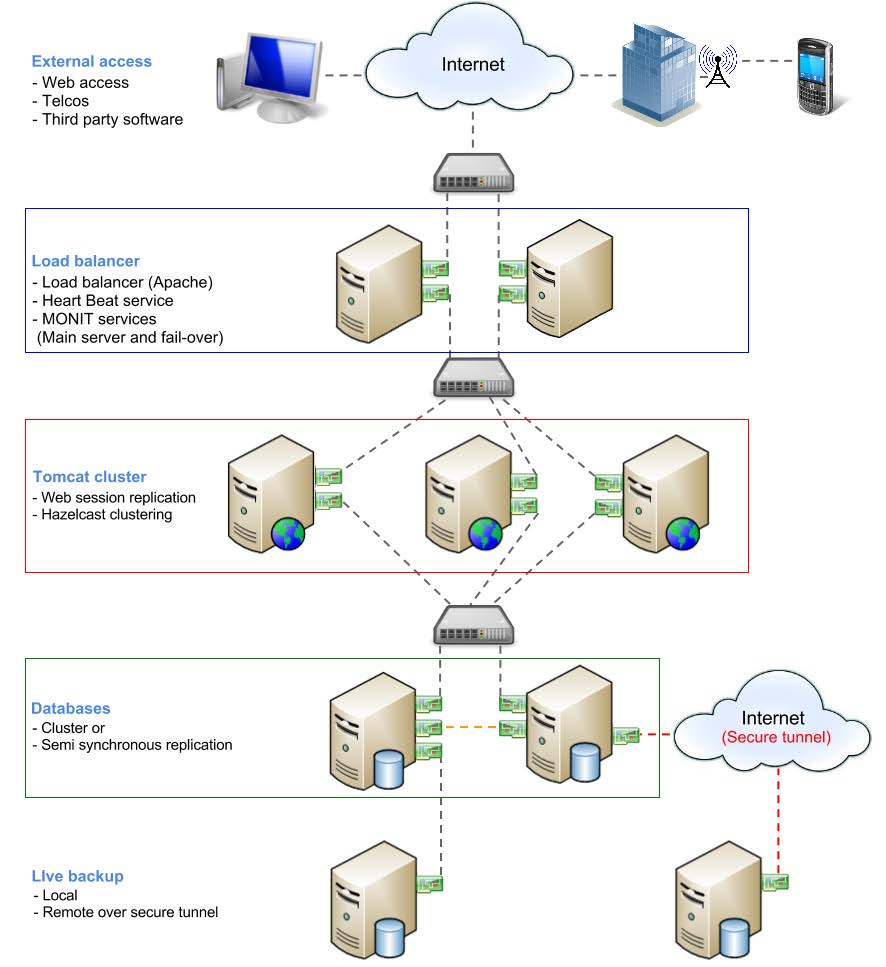
\includegraphics[width=0.7\linewidth]{fig/java-tomcat-clustering}
\caption{Tomcat Clustering}
\label{fig:java-tomcat-clustering}
\end{figure}

\newpage
\begin{figure}[h!]
\centering
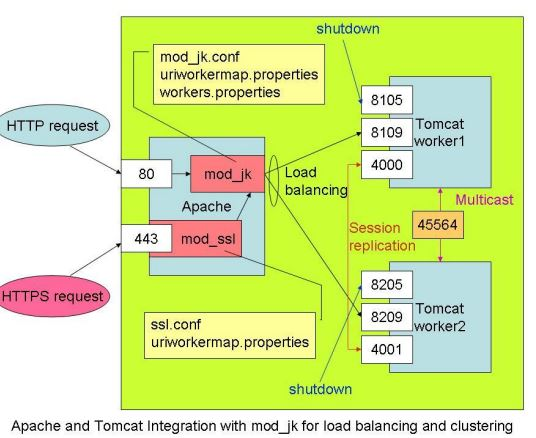
\includegraphics[width=0.7\linewidth]{fig/java-tomcat-mod-jk}
\caption{Tomcat Clustering mod\_jk}
\label{fig:java-tomcat-mod-jk}
\end{figure}

\begin{figure}[h!]
\centering
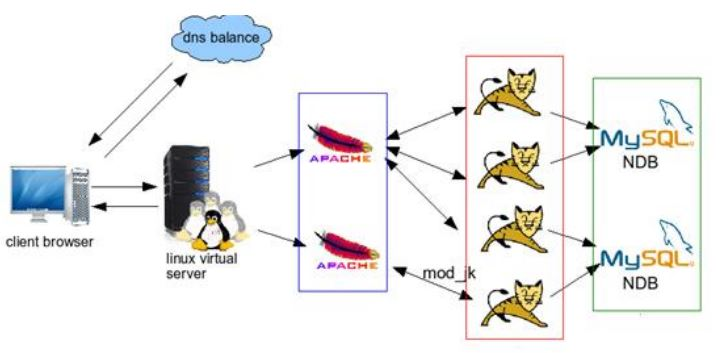
\includegraphics[width=0.7\linewidth]{fig/java-infra}
\caption{Apache + Tomcat + MySQL}
\label{fig:java-infra}
\end{figure}

\newpage
\paragraph{Web-Sockets}
Mit Tomcat 7 werden nun auch WebSockets unterstützt, welches eine full-duplex single socket zwischen Client und Server repräsentiert. Wir kennen die Vorteile von Websockets PUSH instead of POLL.

\begin{figure}[h!]
\centering
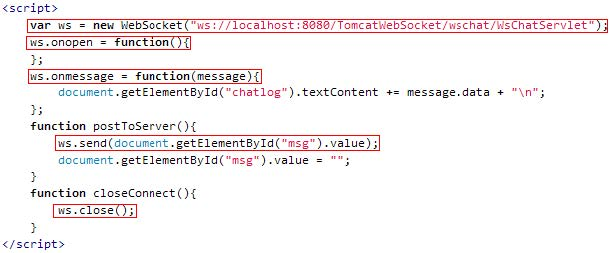
\includegraphics[width=0.7\linewidth]{fig/java-websocket-js}
\caption{Websocket Javascript}
\label{fig:java-websocket-js}
\end{figure}

\begin{figure}[h!]
	\centering
	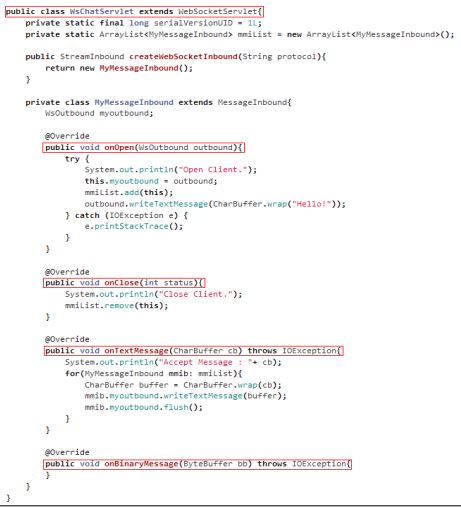
\includegraphics[width=0.6\linewidth]{fig/java-websocket-servlet}
	\caption{Websocket Servlet}
	\label{fig:java-websocket-servlet}
\end{figure}


\newpage
\section{Servlet}
Servlets sind in Java implementierte Anwendungskomponenten, die auf einem Server ausgeführt werden, um dort Anfragen von Clients zu empfangen und zu bearbeiten. Sie erweitern die Funktionalität des Web Servers massiv. Servlets sind Java Klassen welche dynamisch die Requests verarbeiten und eine Response erzeugen, unabhängig vom Protokoll! Das \verb|GenericServlet| hat nur die Methode \verb|service()| und ist somit protokollunabhängig. Das \verb|HttpServlet| ist auf das HTTP Protokoll bezogen und überschreibt \verb|service()| um die definierten HTTP-Verb Methoden aufzurfen (\verb|doGet() doPost()|). Auf der Klasse \verb|HttpServletRequest| kann \verb|getParameter()| aufgerufen werden um an die GET- und POST-Parameter zu gelangen. Servlets müssen innerhalb des Servlet-Containers laufen, welcher den Lebenszyklus der Servlets verwaltet (\verb|init()|, \verb|service()|, \verb|destroy()|).

\paragraph{Servlet-Lebenszyklus}
\begin{description}
	\item[INIT:] Objekt wird beim Laden des Servlet-Containers oder bei der ersten Anfrage erzeugt. Dabei wird die Init-Methode aufgerufen, wobei man DB-Verbindungen herstellen kann oder Konfigurationsdaten laden.
	\item[SERVICE:] Die Anfrage wird in der Service-Methode verarbeitet, welches beim HTTP-Servlet in den HTTP-Verb spezifischen Methoden mündet. Dabei kann auf \verb|ServletRequest| und \verb|ServletResponse| zurückgegriffen werden (bzw. \verb|HttpServletRequest| oder \verb|HttpServletResponse|).
	\item[DESTROY:] Der Servlet-Container entscheiden wann das Servlet eliminiert wird. Die Destroy-Methode wird aufgerufen. Guter Zeitpunkt um DB-Verbindungen zu schliessen.
\end{description}

\paragraph{Servlet-API}
\begin{description}
	\item[HTTPServletRequest:] getQueryString(), getRemoteUser(), getRequestSessionId(), isRequestedSessionIdValid(), getCookies(), getSession(boolean) (false sofern aktuell eine gültige Session besteht sonst wird eine neue Session erzeugt.),  getMethod() (retourniert wie der Request gemacht wurde)
	\item[HTTPServletResponse:]	encodeUrl(String), sendRedirect(String), sendError(int), addCookie(Cookie) (fügt Cookie dem Response an)
\end{description}

\begin{lstlisting}[language=Java, caption=Servlet Sample]
public class ExampleServlet extends HttpServlet {
	public void doGet (HttpServletRequest request,
	HttpServletResponse response)
	throws ServletException, IOException {
		response.setContentType("text/html");
		PrintWriter out=response.getWriter();
		out.println("<html>");
		out.println("<head><title>ExampleServlet</title><head>");
		out.println("<body>");
		out.println("<h1>Testing Servlet zu Testzwecken</h1>");
		out.println("</body></html>");
	}
}
\end{lstlisting}

\paragraph{Struktur eine Web-Applikation}
Die Verzeichnisstruktur ist festgelegt. Das Root-Verzeichnis (Document Root) wird zum 'Context-Path' gemappt. Alles innerhalb des Root-Verzeichnis ausser das WEB-INF Verzeichnis ist von aussen zugreifbar. Das WEB-INF Verzeichnis beinhaltet:
\begin{itemize}
	\item WEB-INF/web.xml - Deployment Descriptor. Hier liegen Meta-Informationen vor.
	\item WEB-INF/classes - Kompilierte Klassen
	\item WEB-INF/lib - Verwendete Bibliotheken der Web-Applikation
\end{itemize}

Anschliessend wird mit dem Deployment Deskriptor und den Servlet Klasse zusammen (und evtl. weiteren benötigten Klassen und Dateien) eine Archiv-Datei erzeugt (.war –Datei). Diese kann anschliessend deployt werden.

\begin{lstlisting}[caption=web.xml Sample]
<web-app xmlns="http://java.sun.com/xml/ns/javaee" xmlns:xsi="http://www.w3.org/2001/XMLSchema-instance" xsi:schemaLocation="http://java.sun.com/xml/ns/javaee http://java.sun.com/xml/ns/javaee/web-app_3_0.xsd" version="3.0">
	<display-name>Tomcat Example Servlet App</display-name>
	<description>A small Example Servlet App</description>
	<servlet>
		<servlet-name>ExampleServlet</servlet-name>
		<servlet-class>ExampleServlet</servlet-class>
	</servlet>
	<servlet-mapping>
		<servlet-name>ExampleServlet</servlet-name>
		<url-pattern>/ExampleServlet</url-pattern>
	</servlet-mapping>
	<welcome-file-list>
		<welcome-file>/pages/ExampleServlet.html</welcome-file>
	</welcome-file-list>
</web-app>
\end{lstlisting}



% Themen:
% done WebAppServer am Beispiel Tomcat
% done WebApp/Servlet Aufbau und Struktur
% done Deployment
% done Beispiele anschauen und nachvollziehen können, Vergleich mit JavaEE

% Dokumente:
% don e05a.Java_im_Webumfeld.pdf
% done 05b.Tomcat_extras.pdf